\chapter{システム構成}

ここでは,PCワークにおける進捗監視システムの処理の流れと,具体的な内容について述べる.
はじめに,システムの概要について述べる.
その後,アプリケーションの機能と,監視方式,そして記録された情報の出力について説明する.

\section{システム概要}
今回提案するシステムの全体を,図\ref{fig:structure_chart}に示す.
本システムでは,最初にPCワークを行うアプリケーション利用者(以下,ユーザ)が作業予定の設定を行う.
設定後,ユーザはアプリケーションをバックグラウンドで起動しながら,作業を行う.
その間,起動中のアプリケーションが,ユーザの作業状況を監視し,記録を行う.
記録された情報は,定期的に作業状況として監督者に通知され,監督者はユーザの行動を把握することができる.

\clearpage

\begin{figure}[h]
  \begin{center}
  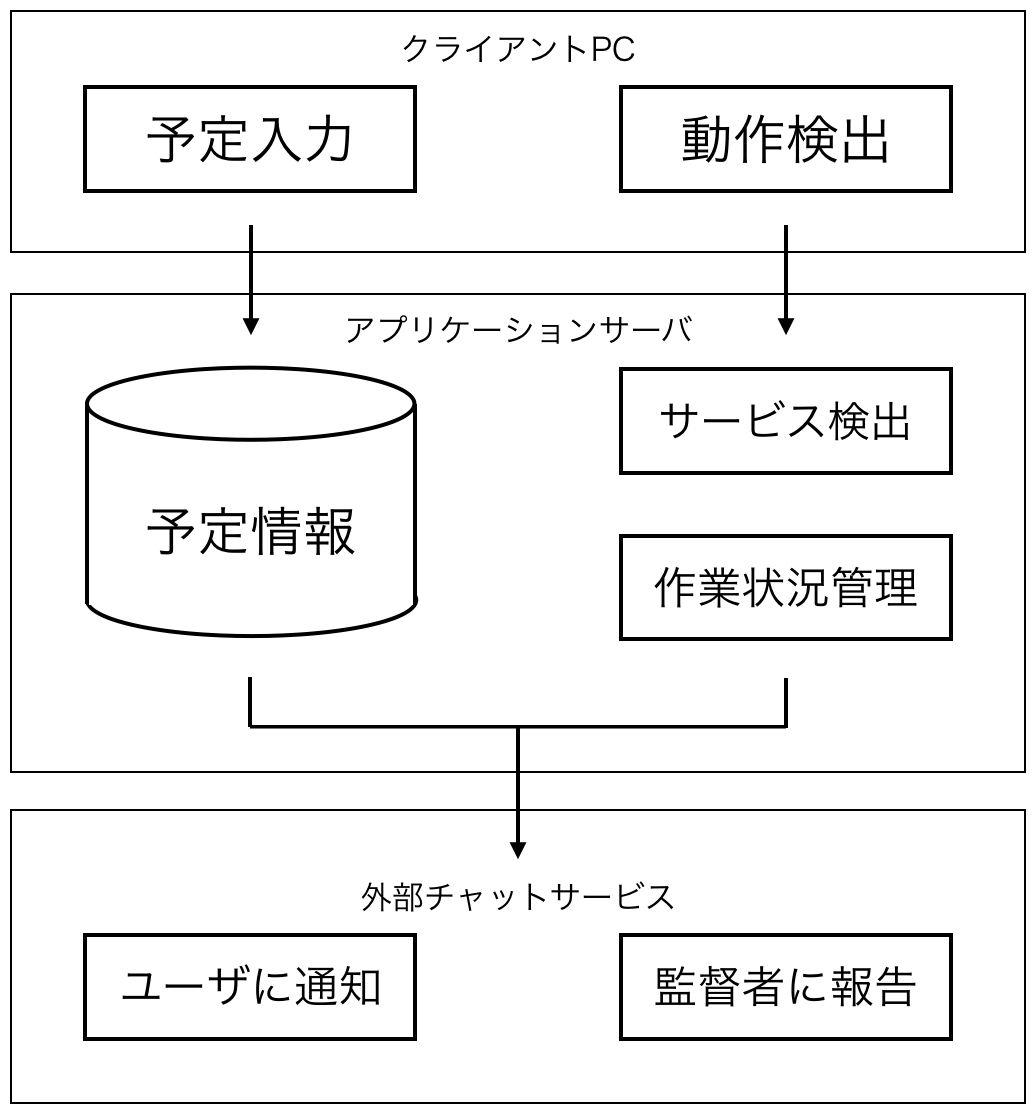
\includegraphics[width=9.0cm]{graphics/structure_chart.png}
  \caption{システム構成図}
  \label{fig:structure_chart}
  \end{center}
\end{figure}

\section{予定の管理機能}
ユーザは,システム利用開始時に,作業予定の設定を行う.設定内容は,作業内容と,作業日時で構成される.
設定された作業予定は,ユーザへの通知や,監督者へ状況を報告する際に利用される.
また,作業全体の進捗状況も,設定された予定が基準になっている.
ユーザはアプリケーション内でいつでも予定を変更することが可能であるが,予定を変更した履歴も監督者に通知される.

\section{アプリケーションによる監視}
本システムでは,アプリケーション内でPCを監視する際,起動状況及び,利用中のサービスの検出を行う.

\subsection{起動状況の記録}
アプリケーションの起動状況は,ユーザがバックグラウンドで起動させている状態で,自動的にサーバに記録される.
また,作業予定になっているもののうち,現在何の作業を行っているのかをユーザが能動的に記録することも可能である.
ただし,自動検知された起動状況は,ユーザ自身が書き換えることはできない.

\subsection{サービス検出}
本研究でのアプリケーションでは,ユーザのPC上で現在表示している画面から,サービスの検出を行う.
まず,アプリケーションが起動している間,ユーザがPC上の画面に出力している情報をキャプチャ画像として自動的に保存する.
その後サーバ上で,それらの画像を解析することにより,ユーザが利用しているサービスの検出を行う.
画像の解析は,Google社のサービスである, Google Cloud Vision API (以下,Vision API)を利用する.

ユーザの画面キャプチャ画像を Vision API に通すことにより,その画像内に含まれるモノ,テキスト情報,サービスのロゴ画像等が検出される.
それらの情報を元に,ユーザが作業に不要なサービスを利用していないかの判別を行う.


\subsection{通知}
アプリケーションからユーザ及び監督者へ通知には,外部のチャットサービスを利用する.
まず,設定された作業予定時に,ユーザに対して通知が送信される.
ユーザは,チャットサービスから受け取る通知により,作業時間であることを認識することができる.
また,1日に1回,決まった時刻に,前日の作業記録を監督者に通知する.
監督者はそれらの記録を確認することにより,ユーザが作業を行った時間や,作業状況を把握することができる.

\clearpage

\section{作業記録の生成}
ユーザは,アプリケーション内で常に自分の作業状況を確認することができる.
作業記録は,主に2種類の形式で生成される.
1つは図\ref{fig:activity_table}のように,作業時間をテーブル上に色分けしたものである.
そのテーブルの上に,作業が行われた時間帯が色分けされる.
テーブルの色分けは以下のように設定した.

\begin{table}[h]
  \begin{tabular}{ll}
    カラーコード & 記録 \\
    ebedf0 & 作業予定時間外 \\
    eeff41 & 作業を行っていた \\
    f9fbe7 & 作業を中断していた \\
    3e2723 & 作業予定時間に,作業ができていなかった \\
  \end{tabular}
\end{table}

\begin{figure}[h]
  \begin{center}
  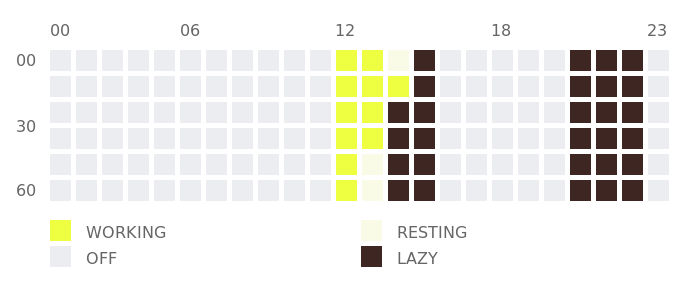
\includegraphics[width=12.0cm]{graphics/activity_table.png}
  \caption{作業時間のテーブル}
  \label{fig:activity_table}
  \end{center}
\end{figure}

\clearpage

もう1つは,ユーザのアプリケーション内の動作を記録した情報である.
図\ref{fig:activity_log}のように,動作の検出時間と,内容をリスト形式で表示する.
これらの作業記録はすべて監督者への通知でも利用される.

\begin{figure}[h]
  \begin{center}
  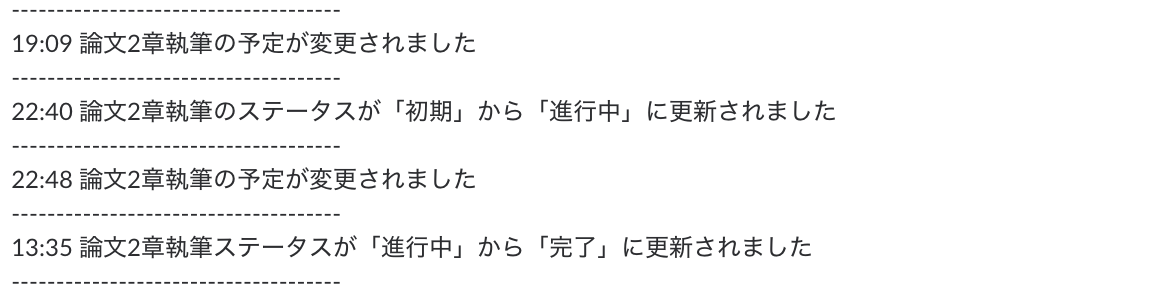
\includegraphics[width=14.0cm]{graphics/activity_log.png}
  \caption{作業時間のテーブル}
  \label{fig:activity_log}
  \end{center}
\end{figure}

%以降削除すること
\clearpage
\noindent
一二三四五六七八九零一二三四五六七八九零一二三四五六七八九零一二三四五\\
二\\
三\\
四\\
五\\
六\\
七\\
八\\
九\\
零\\
一\\
二\\
三\\
四\\
五\\
六\\
七\\
八\\
九\\
零  行数と列数の設定テスト 30行×35文字 = 1050文字/ページ\\
一\\
二\\
三\\
四\\
五\\
六\\
七\\
八\\
九\\
零

